\section{Introduction to C++}

\subsection{C++ language}

\begin{frame}[t]{C++}
\begin{columns}[T]

\column{.5\textwidth}

\begin{itemize}
  \item A \textmark{systems programming} language:
    \begin{itemize}
      \item Lightweight abstractions.
      \item Generates binary code.
      \item Highly efficient.
      \item Used in many domains.
    \end{itemize}

  \mode<presentation>{\vfill\pause}
  \item Multiple \textmark{styles} supported:
    \begin{itemize}
      \item Data abstractions.
      \item Object oriented programming.
      \item Generic programming.
      \item Functional programming.
      \item Asyncrhonous programming.
      \item Concurrency.
    \end{itemize}
\end{itemize}

\column[T]{.5\textwidth}

\pause
\vspace{-1em}
\begin{center}
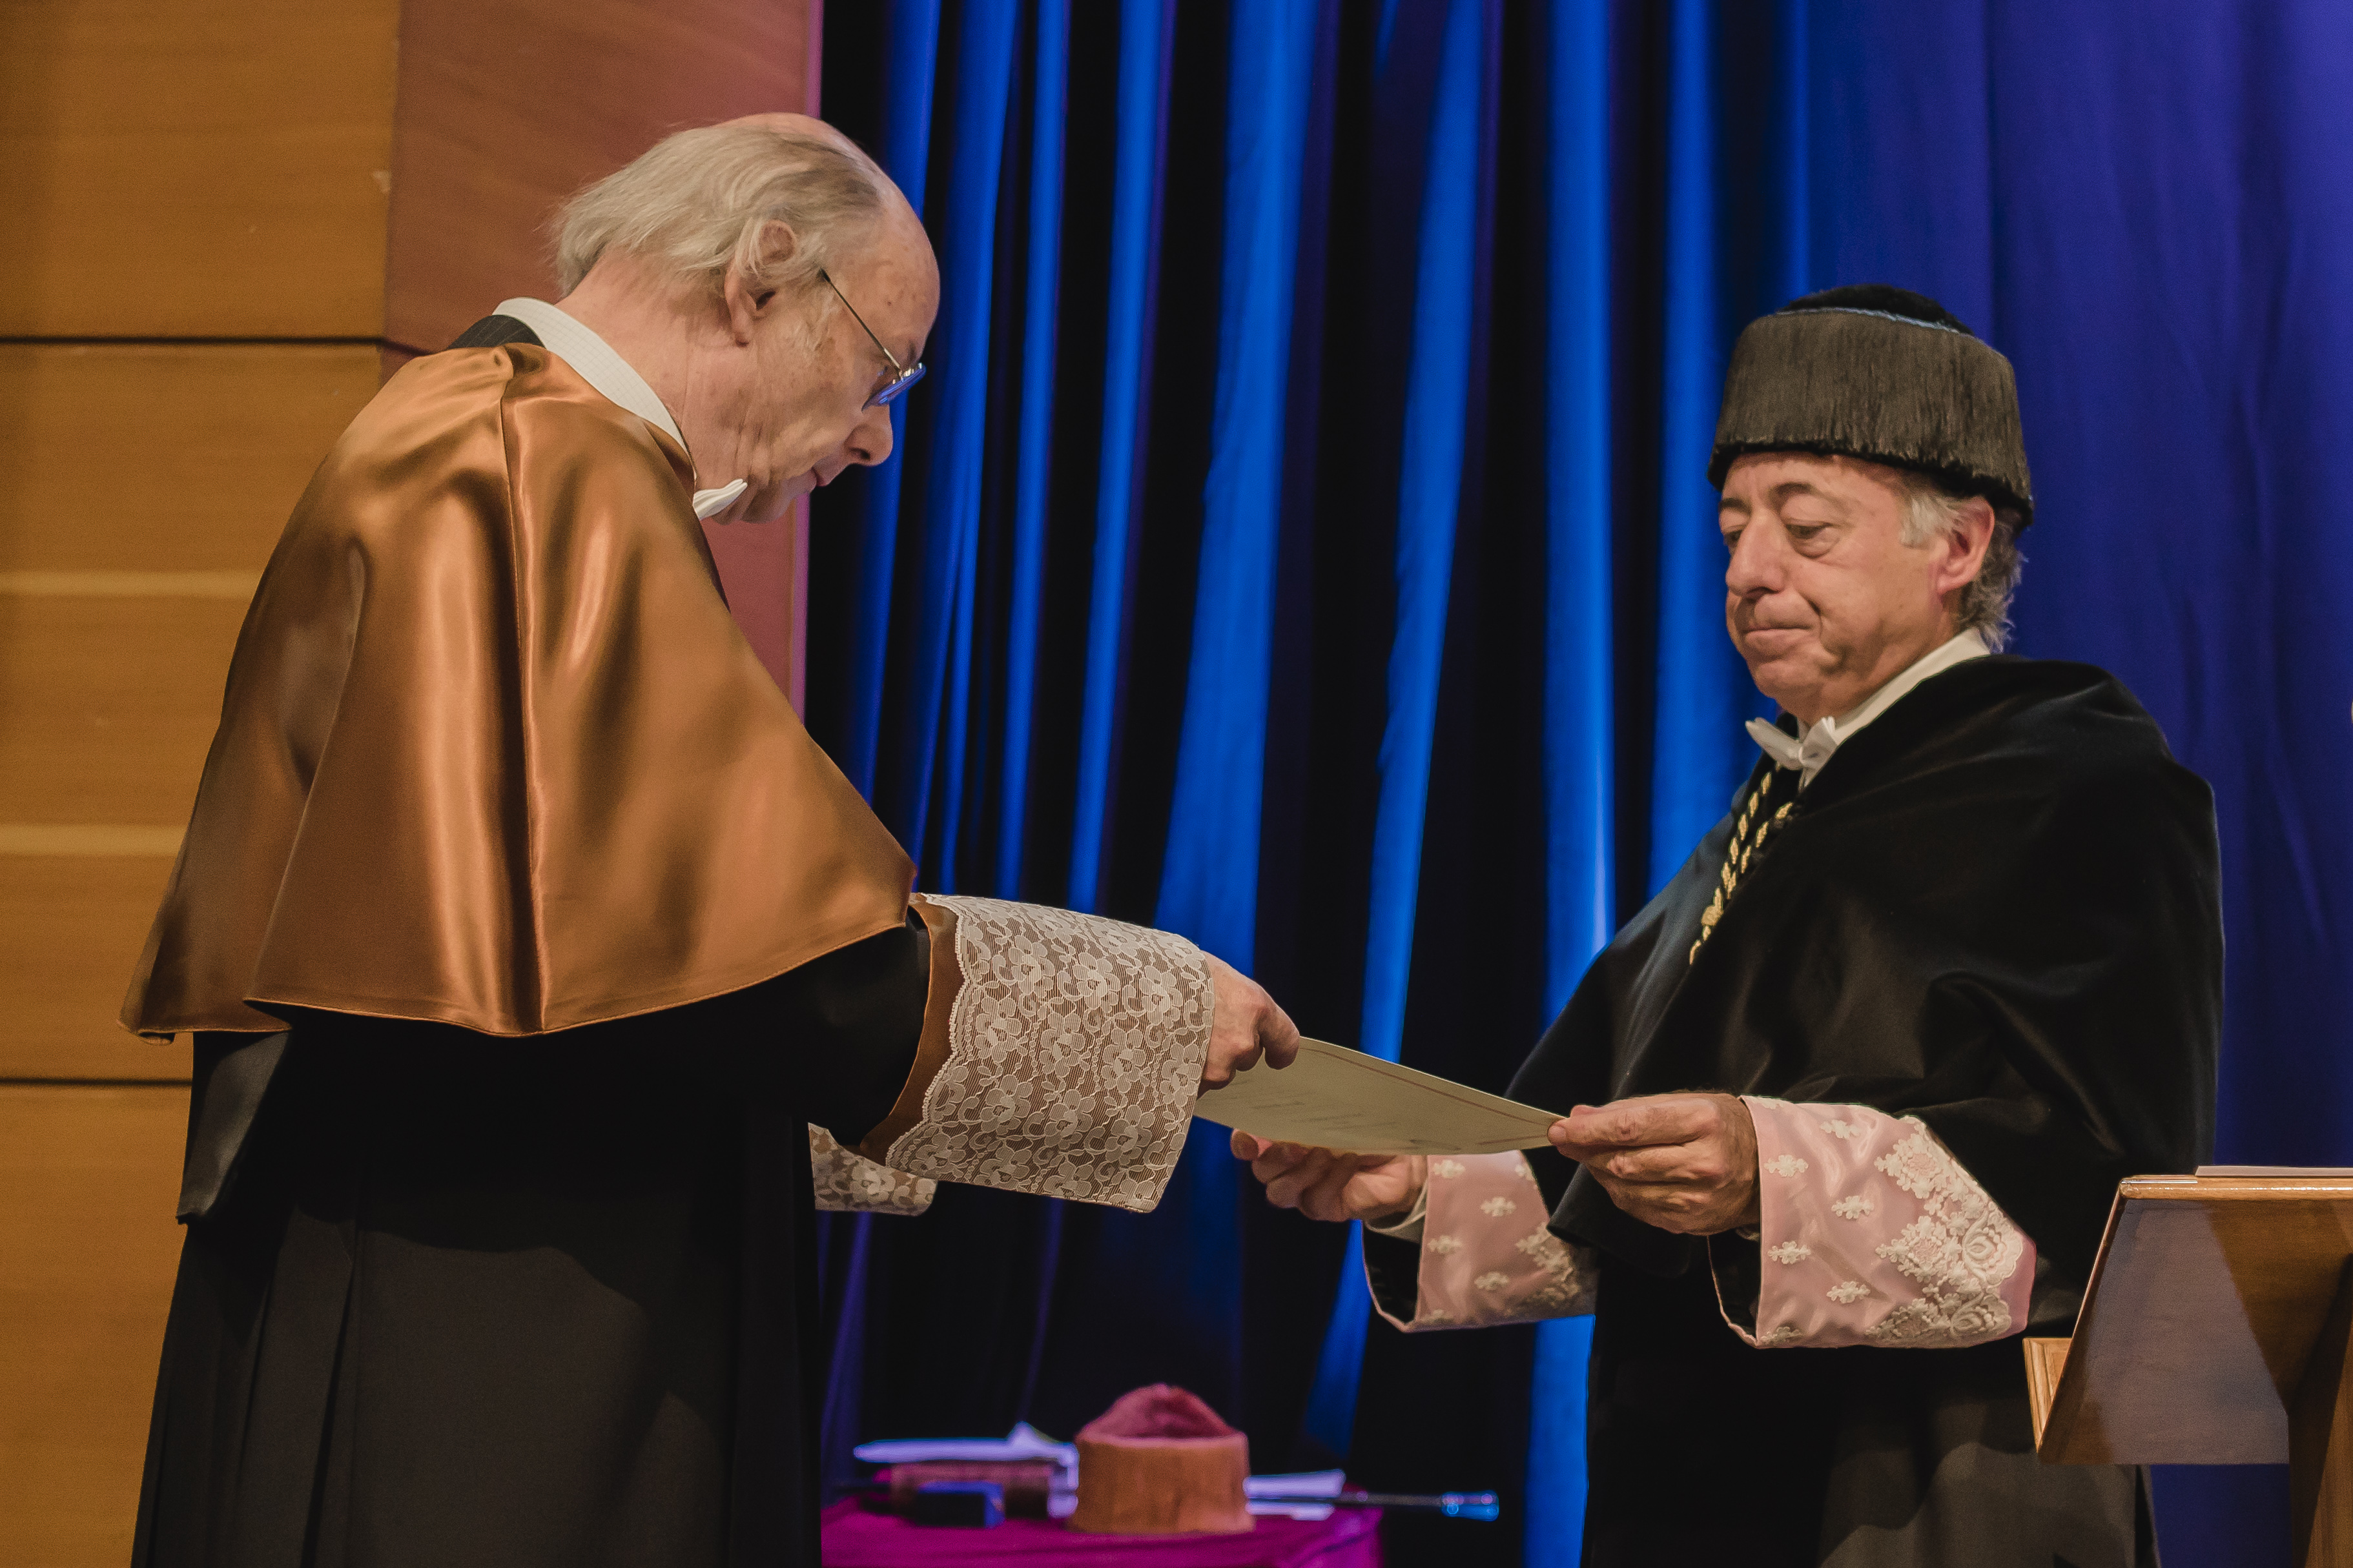
\includegraphics[width=.5\textwidth]{images/bjarne-honoris.jpg}
\end{center}

\begin{itemize}
  \item Designed by \textgood{Bjarne Stroustrup}.
\end{itemize}

\pause

\includegraphics[width=.5\textwidth]{images/logo-iso.png}

\includegraphics[width=.2\textwidth]{images/logo-cpp.png}

\begin{itemize}
  \item ISO/IEC 14882 series.
\end{itemize}


\end{columns}
\end{frame}
